\documentclass{beamer}
\usetheme{Zurich}
\usepackage{amsmath, amsfonts, graphicx, multirow}
\title{Classification and Regression Trees}
\author{Charlotte Wickham}
\date{\today}

\begin{document}

\frame{\titlepage}

\section[Outline]{ 	}
\frame{\tableofcontents}

\begin{frame}
	\frametitle{}
	\begin{columns}[c] 
		\column{.6\textwidth} 
			\setkeys{Gin}{width=\textwidth}
			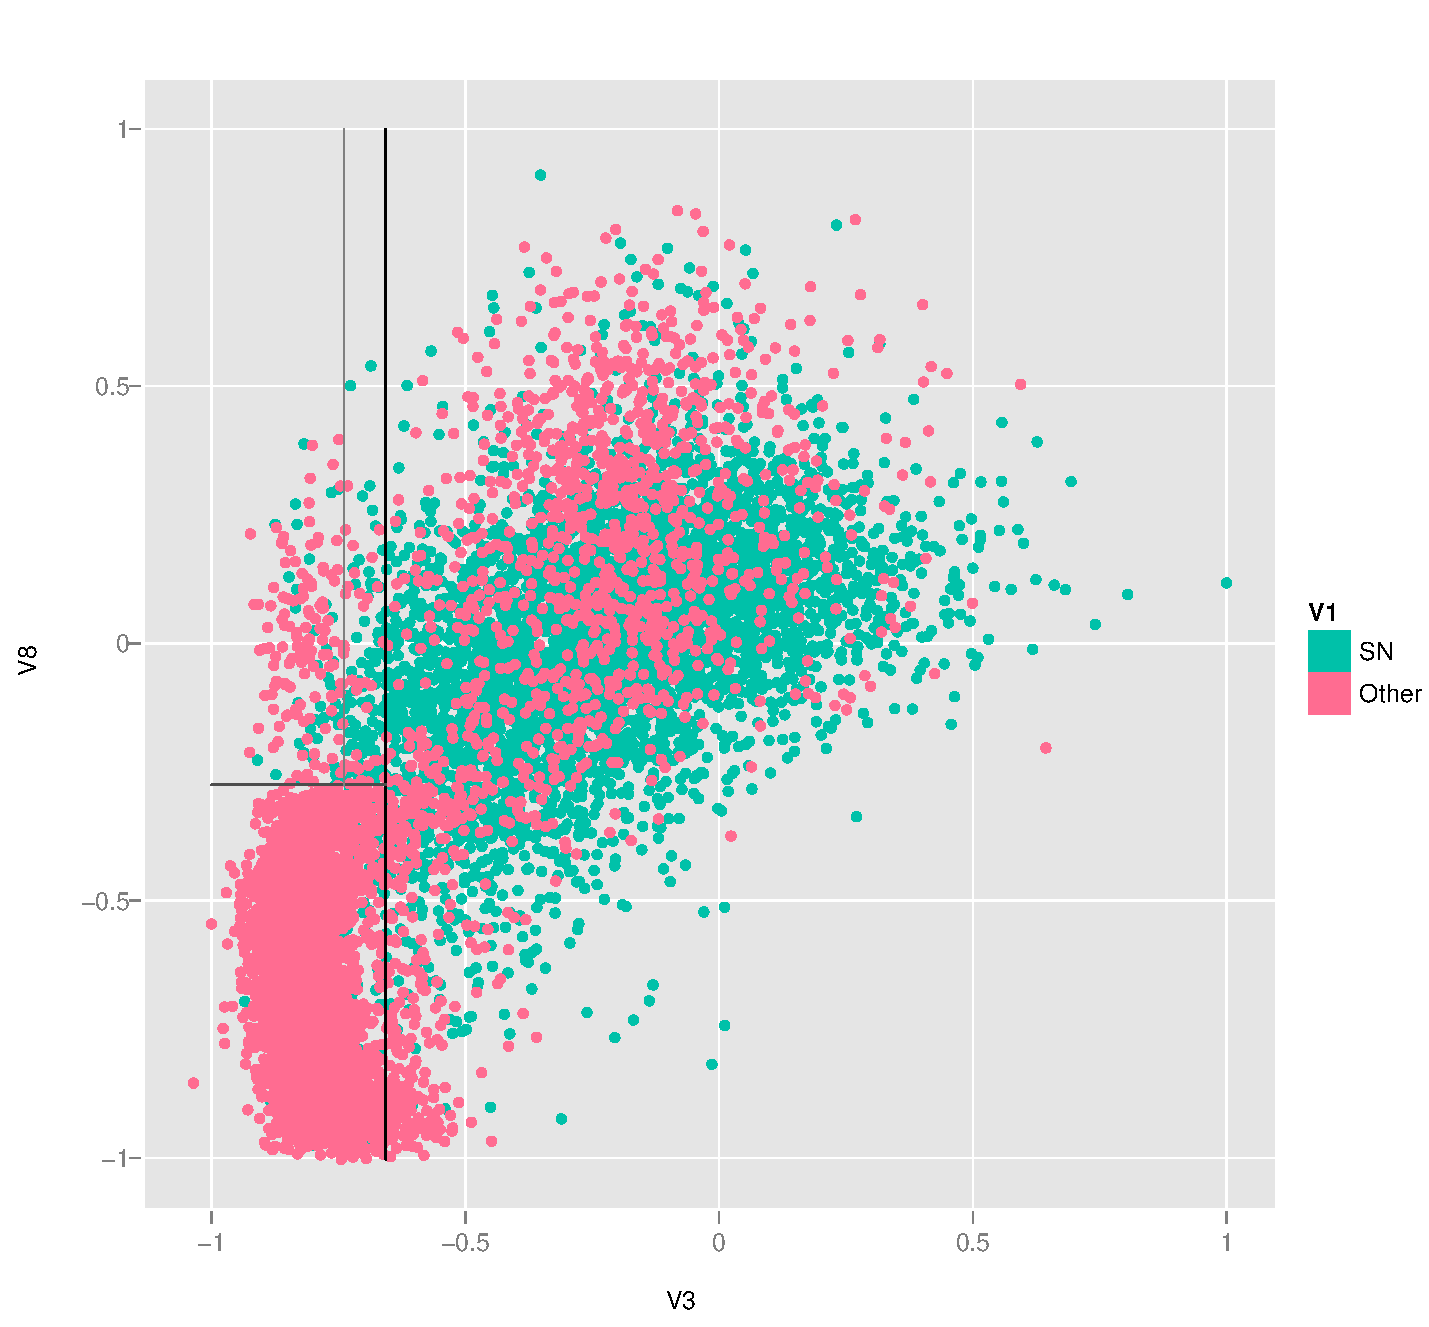
\includegraphics{leftside.pdf}
		\column{.4\textwidth}
			Splits on two variables classified a lot of the ``Other'' objects.
			They were:
			\begin{itemize}
				\item perinc (V3) - \% flux increase in aperture from REF to NEW 
			 	\item neighbordist (V8) - distance to the nearest object in REF 
			\end{itemize}		
	\end{columns}
	\end{frame}

\section{Details from last week}
\subsection{rpart}
\begin{frame}
	\frametitle{rpart}
	\begin{itemize}
		\item Does not use balanced cross-validation sets.
		\item rpart's \texttt{cp} parameter
		\[
			R_{cp}(T) = R(T) + cp \times |T| \times R(T_0)
		\]
		where $T_0$ is the tree with no splits. 	(Recall $R(T) =$ misclassification rate of tree $T$.)
		\item in CART
		\[
		R_\alpha = R(T) + \alpha \times |T|.
		\]
		So the tree than minimizes $R_{cp}$ is the same as that which minimizes $R_{\alpha = cp\times R(T_0)}$.
	\end{itemize}
\end{frame}

\begin{frame}
\frametitle{Pruning}
\begin{columns}[c] % the "c" option specifies center vertical alignment 
	\column{.6\textwidth} % column designated by a command
\setkeys{Gin}{width=\textwidth}
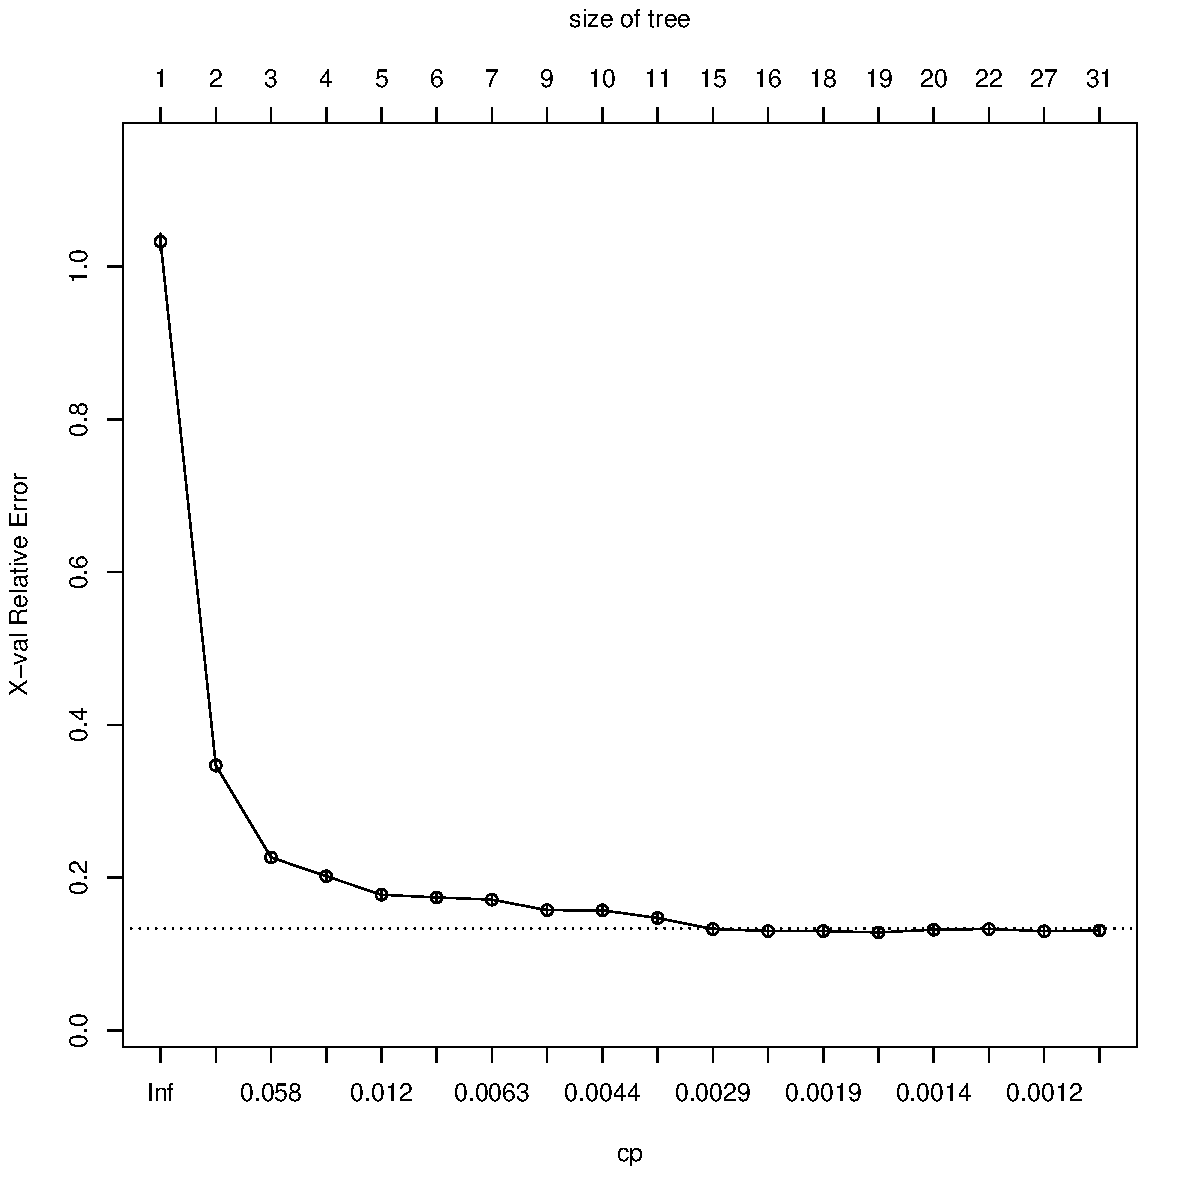
\includegraphics{cp.pdf}
	\column{.4\textwidth}
	\end{columns}
\end{frame}

\subsection{Priors and Costs}
\begin{frame}
	\frametitle{Priors and Costs}
	May have prior probabilities for each class $\pi_i, \quad i=1,\ldots, C$. 
	
	May also have cost for misclassifying an $i$ as a $j$, $L(i,j)$.
	
	Where do these enter the growth and pruning of trees?
	\begin{itemize}
		\item In splitting
		\item In pruning
		\item In class assignment
		\begin{itemize}
			\item Now terminal nodes are assigned to class $i$ where $i$ minimizes
			\[
			\sum_j{C(i|j)p(j|t)}.
			\]
		\end{itemize}
	\end{itemize}

\end{frame}

\begin{frame}
	\frametitle{Priors}
	Have $\pi_i, \quad i=1,\ldots,J \quad \sum_{i=1}^J \pi_i = 1$. Let $N_j(t)$ be the number of cases of class $j$ falling into node $t$.  Then,
	\[
		p(j,t) = \pi(j)N_j(t)/N_j
	\]
	is the estimate for the probability of a case will be type $j$ and fall into node $t$. 
	\[
		p(t) = \sum_j p(j,t)
	\]
	is the estimate for the probability that any case will fall into node $t$. 
	
	\[
		p(j|t) = p(j,t)/p(t)
	\]
	is the estimate for the probability of a case will be type $j$ given it falls into node $t$. 
	
\end{frame}

\begin{frame}
	\frametitle{Priors in splitting}
	Let the impurity of a node $t$ be, 
	\[
	I(t) = \sum_{i\ne j}p(i|t)p(j|t), \text{ (Gini index)}.
	\]
	And we are choosing split, $s$, to minimise,
	\[
	\Delta I(s,t) = I(t) - p_RI(t_R) - p_LI(t_L)
	\]
	where $p_R = p(t_R)/p(t)$ and $p_L$ similarly.
	
	So, the priors affect splitting by simply adjusting the estimated proportions ($p(i|t)$, $p_R$, etc) needed to calculate the impurity.
	
	Note the classification cost doesn't come in here.
\end{frame}

\begin{frame}
	\frametitle{Including misclassification costs in splitting}
	Two methods.  First,
	\begin{itemize}
		\item Generalized Gini impurity 
				\[
				I(t) = \sum_{j, i}C(i|j)p(i|t)p(j|t),
				\]
			\begin{itemize}
				\item Only depends on symmetrized cost matrix
				\item Might not be concave in $\{p(j|t)\}$ so decrease in impurity could be negative.
			\end{itemize}
	
	\end{itemize}
\end{frame}

\begin{frame}
	\frametitle{Including misclassification costs in splitting}
	Second,
	\begin{itemize}
		\item Altered priors
		\begin{itemize}
			\item Priors and costs are somewhat interchangeable
			\item Let $Q(i|j)$ be the proportion of class $i$ classified as class $j$ by tree $T$.  Then the estimate of misclassification is
			\[
			R(T) = \sum_{i,j} C(i|j)Q(i|j)\pi(j)
			\]
			\item Can find $C'(i|j)$ and $\pi'(j)$ such that R(T) doesn't change.
			\item In the case that $C(i|j) = C(j) \quad i\ne j$, let $C'(i|j)$ be unit costs and define 
			\[
			\pi'(j) = C(j)\pi(j)/\sum_j C(j)\pi(j)
			\]
			\item Use these altered priors as per usual.
		\end{itemize}
	\end{itemize}
\end{frame}

\begin{frame}
	\frametitle{Pruning}
		Cost-complexity pruning
		\begin{itemize}
			\item Choose tree $T$ that minimizes,
			\[
			R_\alpha(T) = R(T) + \alpha |\widetilde{T}|,
			\]
			$|\widetilde{T}| =$ the number of terminal nodes of $T$.
			\item Priors and costs come into definition of R(T), the misclassification cost of $T$ (or the risk).
			\[
			R(T) = \sum_{t\in\widetilde{T}}R(t)
			\]
			\begin{eqnarray*}
			R(t) &=& r(t)p(t) \\
			&=& \left(\min_i \sum_j C(i|j)p(j|t) \right) p(t)
			\end{eqnarray*}
		\end{itemize}
\end{frame}

\begin{frame}
	\frametitle{Costs and priors in supernova data}
	\begin{itemize}
		\item Raquel says more than 10,000 negatives for every positive.
		\item so try prior $P(\text{sn}) = 1/10000$ $P(\text{other}) = (10000-1)/10000$.
		\item no cost
		\item Didn't work so well
	\end{itemize}
\end{frame}

\begin{frame}
	\frametitle{Priors in supernova data}
	\begin{columns}[c] 
		\column{.6\textwidth} 
			\setkeys{Gin}{width=\textwidth}
			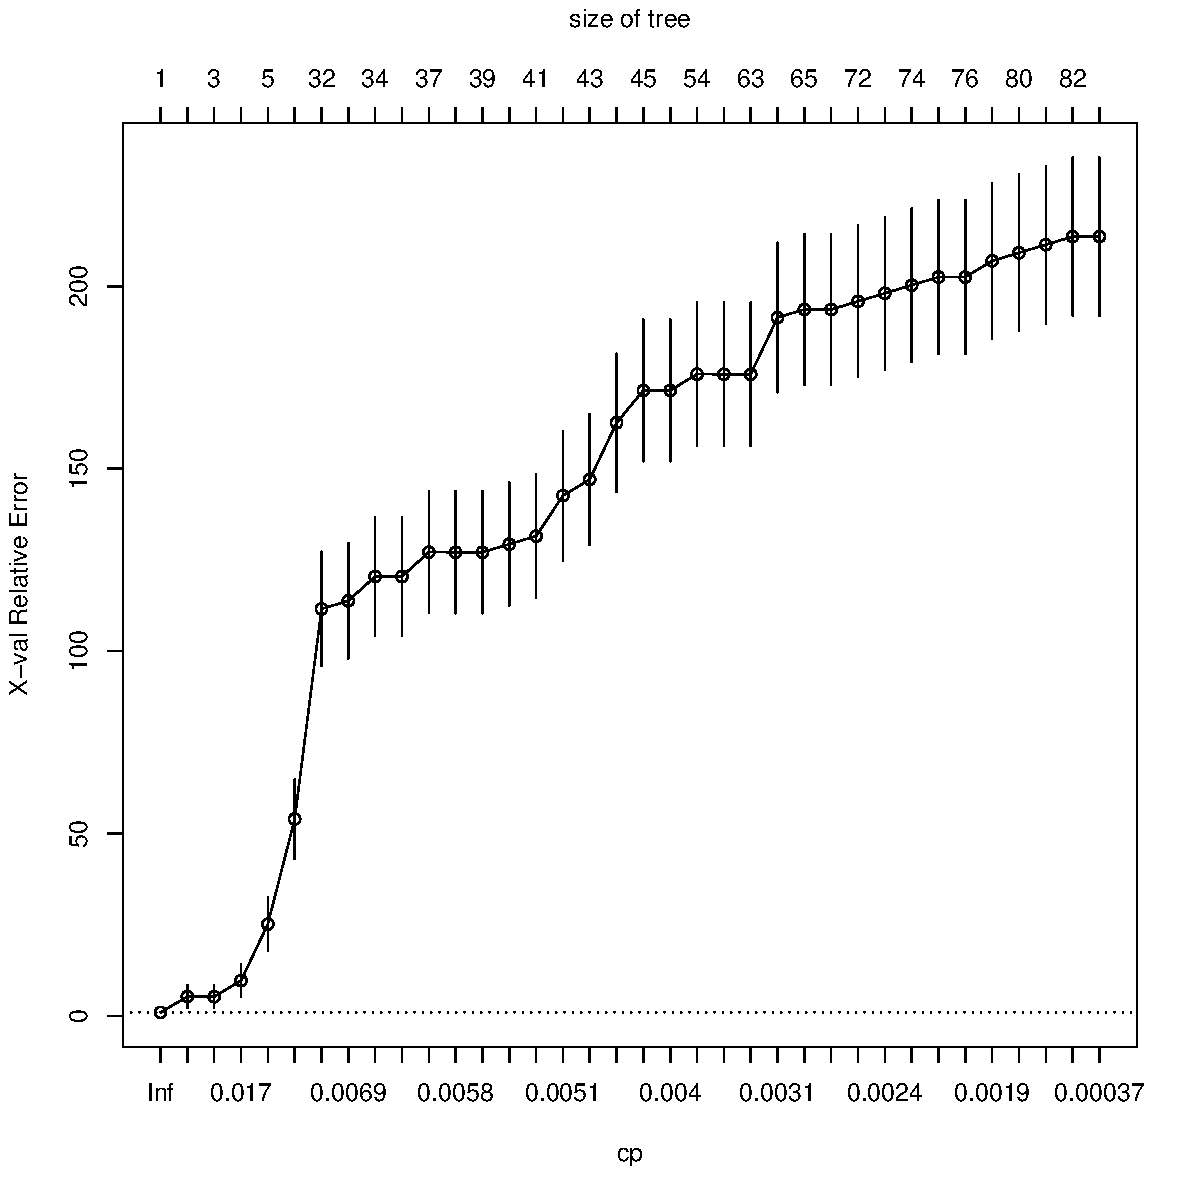
\includegraphics{cpp1.pdf}
		\column{.4\textwidth}
			\begin{itemize}
				\item Error gets bigger as tree grows?
			\end{itemize}
	\end{columns}
\end{frame}

\begin{frame}
	\frametitle{Costs and priors in supernova data}
	\begin{itemize}
		\item Try something a little more moderate.
		\item Still no good if $P(\text{sn}) = 1/100$ $P(\text{other}) = 99/100$.
		\item So try prior $P(\text{sn}) = 1/10$ $P(\text{other}) = 9/10$.
	\end{itemize}
\end{frame}

\begin{frame}
	\frametitle{Priors in supernova data}
	\begin{columns}[c] 
		\column{.6\textwidth} 
			\setkeys{Gin}{width=\textwidth}
			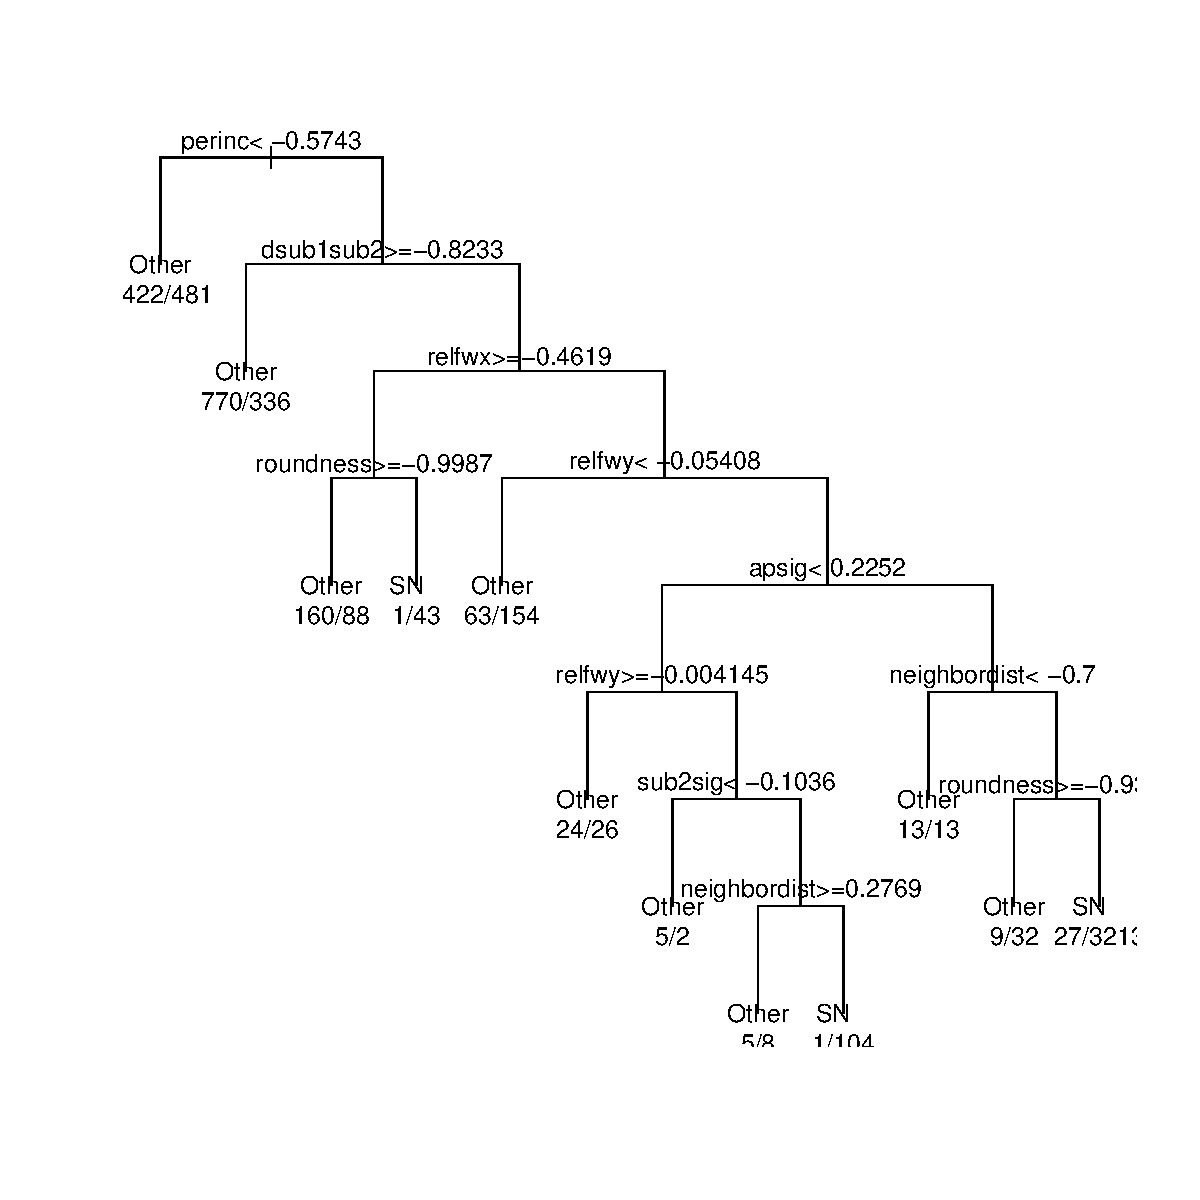
\includegraphics{treep3.pdf}
		\column{.4\textwidth}
				\begin{table}
				\begin{tabular}{cr|rr}
				& & \multicolumn{2}{c}{Prediction}\\
				& & Other & SN\\
				\hline
				\multirow{2}{*}{\rotatebox{90}{Actual}} & Other &  494 &  6\\
				& SN & 142 &  358\\
				\end{tabular}
				\end{table}	
				Total error = 14.8\%
				
				+ve's = 28.4\%
				
				-ve's = 1.2 \%\\\
				
				(Compare with
				
				Total error = 8.4\%
				
				+ve's = 9\%
				
				-ve's = 7.8 \%
			
				when no priors.
				)
			\end{columns}
\end{frame}

\begin{frame}
	\frametitle{Priors in supernova data}
	Also try, $P(\text{sn}) = 3/10$ $P(\text{other}) = 7/10$.
	\begin{columns}[c] 
		\column{.6\textwidth} 
			\setkeys{Gin}{width=\textwidth}
			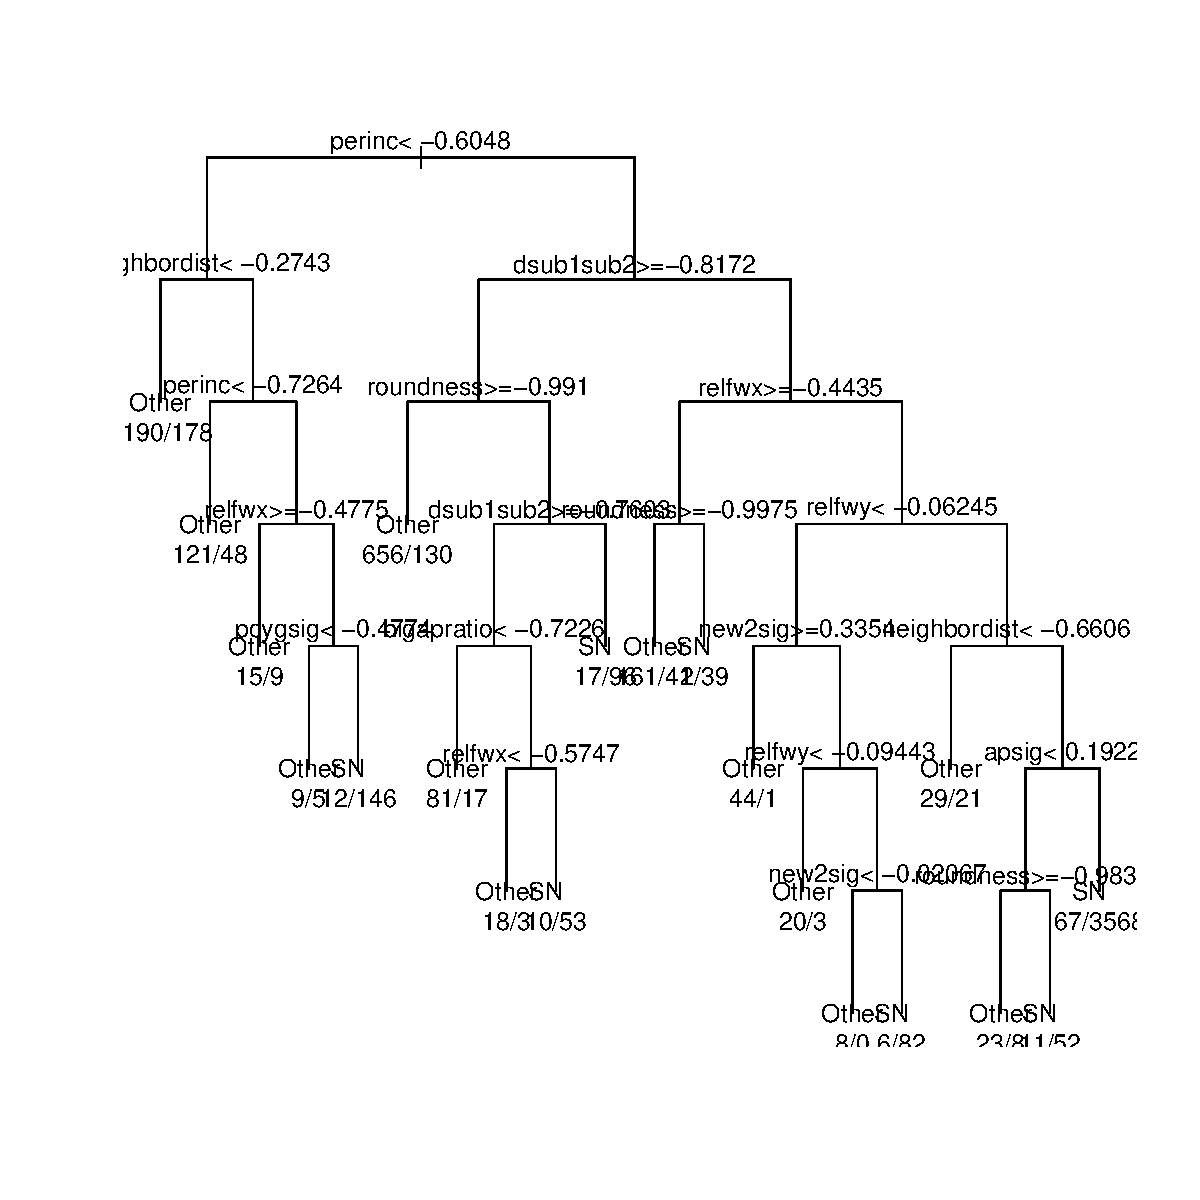
\includegraphics{treep4.pdf}
		\column{.4\textwidth}
				\begin{table}
				\begin{tabular}{cr|rr}
				& & \multicolumn{2}{c}{Prediction}\\
				& & Other & SN\\
				\hline
				\multirow{2}{*}{\rotatebox{90}{Actual}} & Other &  470 &  30\\
				& SN & 59 &  441\\
				\end{tabular}
				\end{table}	
				Total error = 8.9\%
				
				+ve's = 11.6\%
				
				-ve's = 6\%
			\end{columns}
\end{frame}

\begin{frame}
	\frametitle{Costs in supernova data}
	Try costs instead: $C(SN|Other)=2, C(Other|SN)=1$
	\begin{columns}[c] 
		\column{.6\textwidth} 
			\setkeys{Gin}{width=\textwidth}
			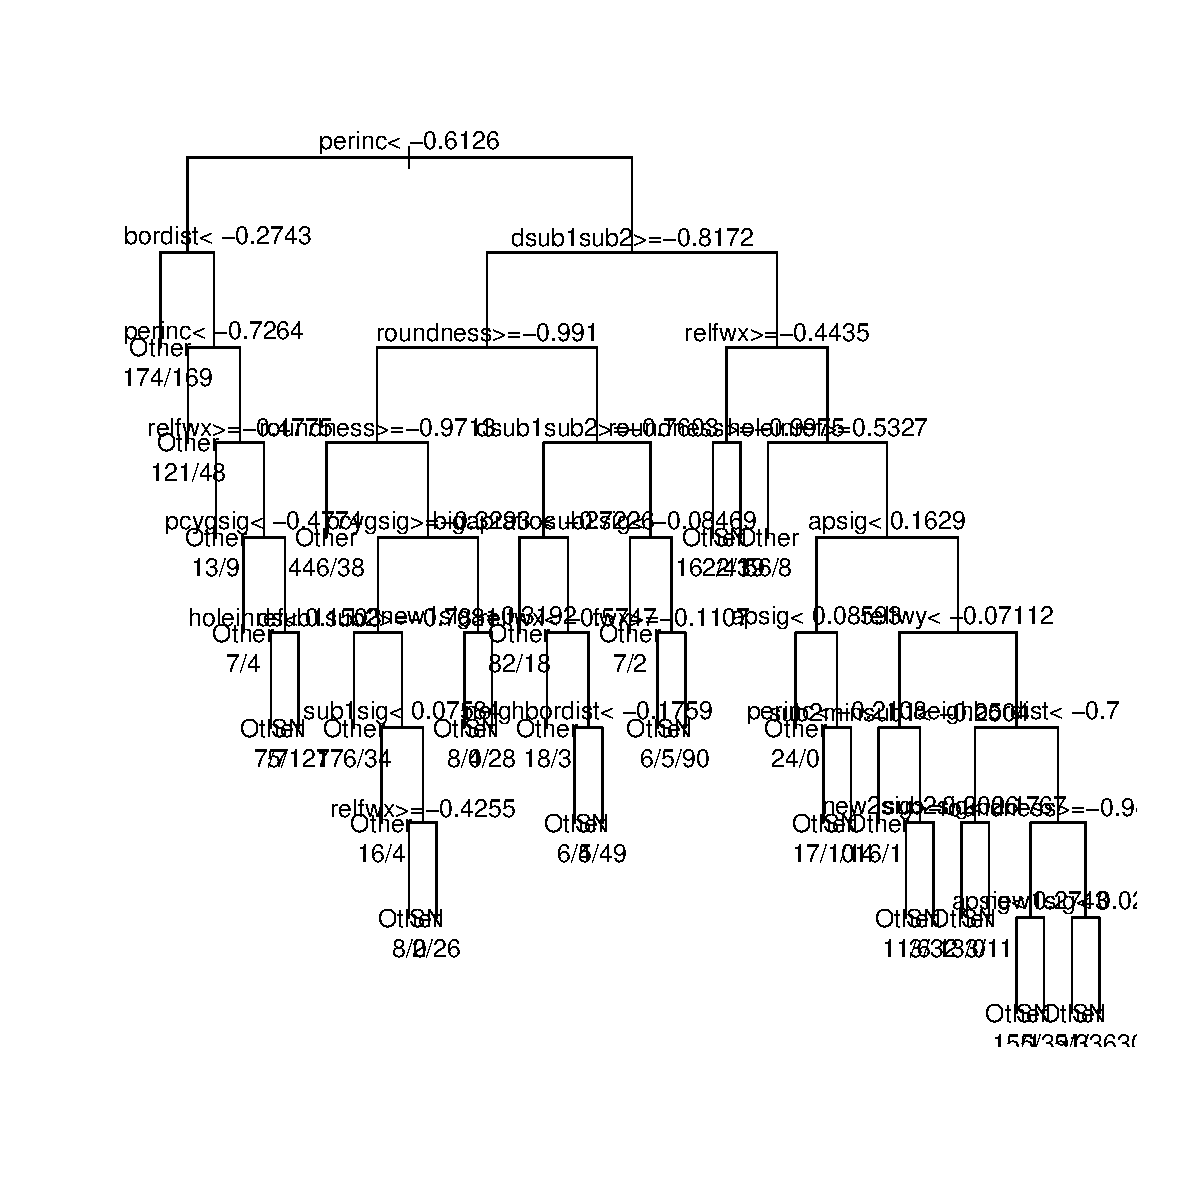
\includegraphics{treec1.pdf}
		\column{.4\textwidth}
				\begin{table}
				\begin{tabular}{cr|rr}
				& & \multicolumn{2}{c}{Prediction}\\
				& & Other & SN\\
				\hline
				\multirow{2}{*}{\rotatebox{90}{Actual}} & Other &  476 &  24\\
				& SN & 55 &  445\\
				\end{tabular}
				\end{table}	
				Total error = 7.9\%
				
				+ve's = 11\%
				
				-ve's = 4.8\%
			\end{columns}
\end{frame}

\begin{frame}
	\frametitle{Costs in supernova data}
	Also try: $C(SN|Other)=3, C(Other|SN)=1$
	\begin{columns}[c] 
		\column{.6\textwidth} 
			\setkeys{Gin}{width=\textwidth}
			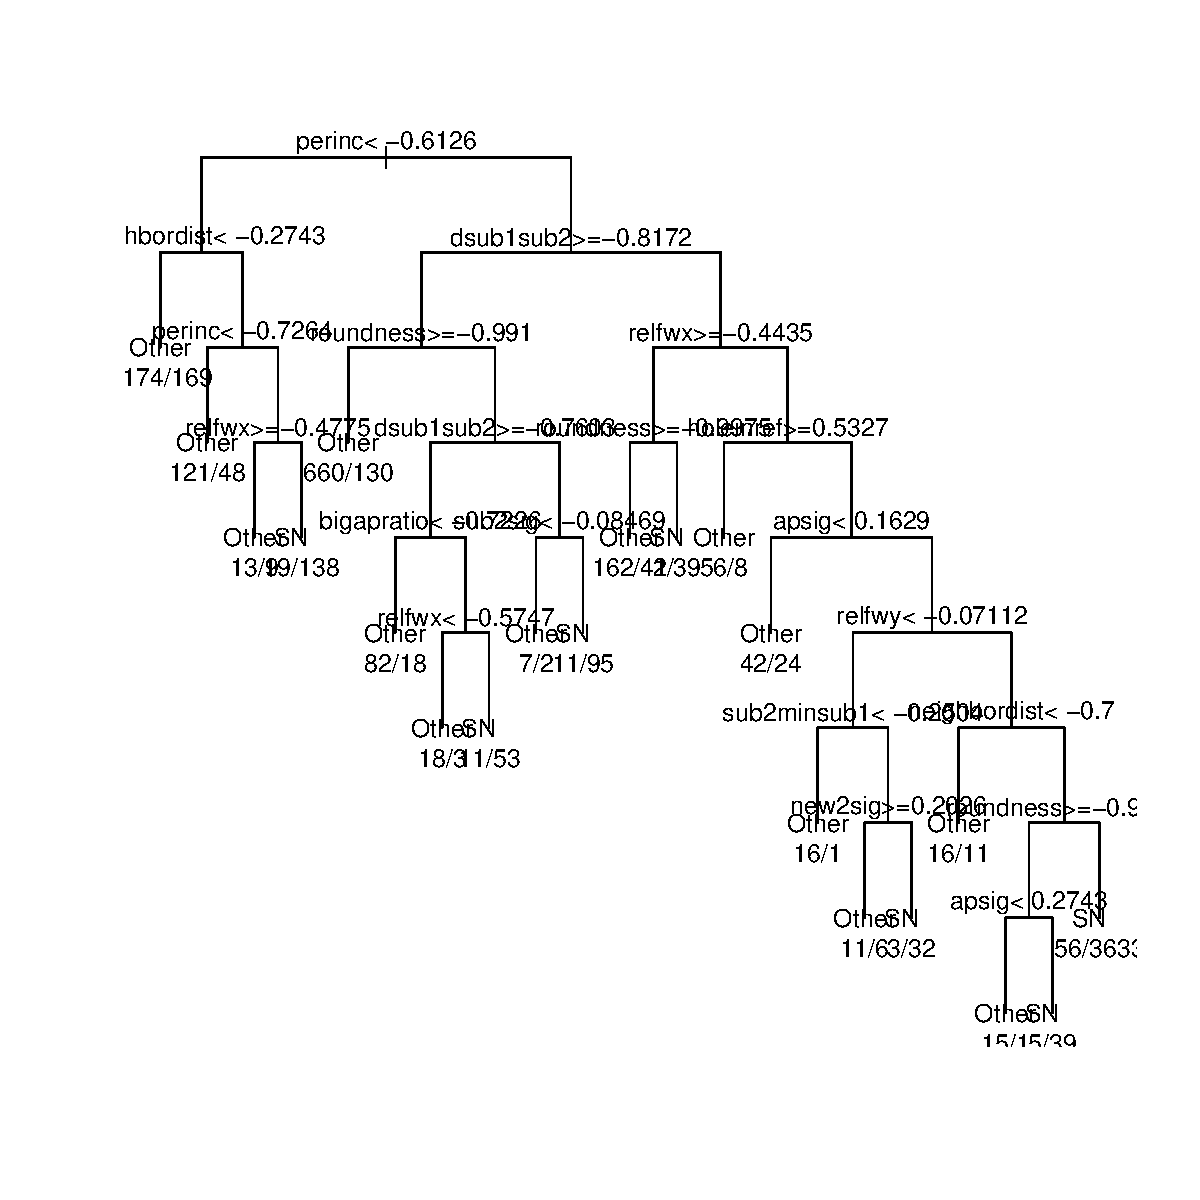
\includegraphics{treec2.pdf}
		\column{.4\textwidth}
				\begin{table}
				\begin{tabular}{cr|rr}
				& & \multicolumn{2}{c}{Prediction}\\
				& & Other & SN\\
				\hline
				\multirow{2}{*}{\rotatebox{90}{Actual}} & Other &  475 &  25\\
				& SN & 56 &  444\\
				\end{tabular}
				\end{table}	
				Very similar to previous.
			\end{columns}
\end{frame}

\subsection{Regression Trees}
\begin{frame}
	\frametitle{Regression Trees}
	\begin{itemize}
		\item Simpler than classification trees since the same measure can be used for splitting and pruning.
		\item Now learning sample consists of $(y_1, \pmb{x_1}), \ldots, (y_n, \pmb{x_n})$. For new $\pmb{x'}$ we want to predict $y'$.
		\item Define our error measure (equivalent to impurity and misclassification measures in classification) as
		\[
		R(t) = \frac{1}{N}\sum_{x_n \in t} (y_n - \bar{y}(t))^2
		\]
		where $\bar{y}(t)$ is the average of all cases in node $t$.
		\item Like the sum of squares within a node.
	\end{itemize}
\end{frame}
\begin{frame}
	\frametitle{Regression cont...}
	\begin{itemize}
		\item Then similarly to the classification case, choose split s which maximises 
		\[
		\Delta R(s,t) = R(t) - R(t_L) - R(t_R)
		\]
		\item Again, grow a large tree and then prune back.
		\item Cost complexity measure,
		\[
		R_\alpha(T) = R(T) + \alpha |\widetilde{T}| \quad \text{where } R(T) = \sum_{t \in \widetilde{T}} R(t)
		\]
		\item Find subset of trees that minimise $R_\alpha$ for various $\alpha$.  Choose good $\alpha$ by cross validation.
		\item 
		Terminal nodes are assigned the value $\bar{y}(t)$ the average value of the cases in the node.
	\end{itemize}
	
\end{frame}
\begin{frame}
	\frametitle{Least deviation regression}
	Previous slides describe least squares regression trees.
	Alternatively, define 
	\[
	R(t) = \frac{1}{N}\sum_{x_n \in t} |(y_n - \nu(t))|
	\]
	where $\nu(t)$ is any median of the cases in node $t$.
	Then terminal nodes are assigned the value $\nu(t)$.
	Can be less sensitive to outliers.
\end{frame}

\begin{frame}
	\frametitle{Diamond Data}
	Measurements of 53935 diamonds and their selling price. 
\begin{tabular}{lp{8cm}}
\hline
Variable & Description\\
\hline
price & Selling price\\
carat & weight of the diamond\\
cut & Fair, Good,  Very Good, Premium, Ideal.\\
color & graded on a letter scale from D to Z. Only D-J in this dataset.\\
clarity & From good to bad:IF, VVS1, VVS2, VS1, VS2, SI1, SI2, I1. \\
totaldepth &  \multirow{5}{*}{Physical dimensions}\\
table & \\
width &\\
height &\\
depth &\\
\hline
\end{tabular}
\end{frame}

\begin{frame}[fragile]
	\frametitle{Best Linear Model}
	\begin{tiny}
	\begin{verbatim}
		Call:
		lm(formula = log(price) ~ carat + cut + color + clarity + totaldepth + 
		    table + width + height + depth, data = dia.train)

		Residual standard error: 0.1353 on 48502 degrees of freedom
		  (16 observations deleted due to missingness)
		Multiple R-Squared: 0.9822,     Adjusted R-squared: 0.9822 
		F-statistic: 1.165e+05 on 23 and 48502 DF,  p-value: < 2.2e-16 
	\end{verbatim}
	
	\end{tiny}	
	Look at MSE on test set for \verb|price|.
	MSE (on original scale) = 309308.8
	
\end{frame}

\begin{frame}
	\frametitle{Regression Tree for diamonds data}
	\begin{columns}[c] 
		\column{.6\textwidth} 
			\setkeys{Gin}{width=\textwidth}
			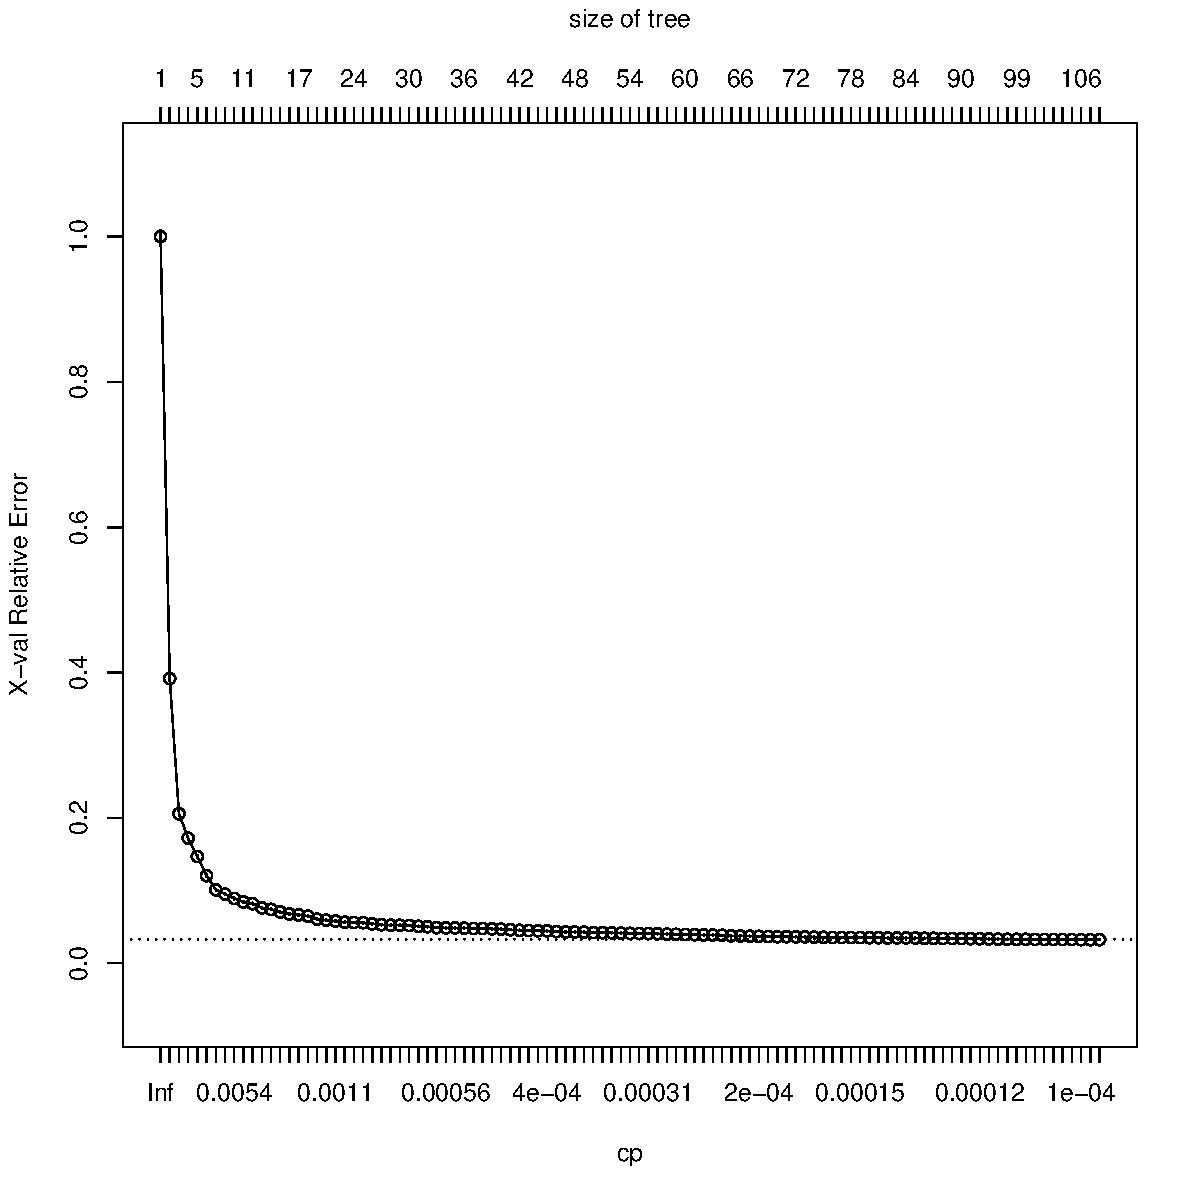
\includegraphics{cpdia.pdf}
		\column{.4\textwidth}
			\begin{itemize}
				\item Decreasing very quickly at first and then very slowly
				\item Try a couple of prunes and check out their performance.
				\item Prune to size 99
				MSE =  218485.4
				
				\item Prune to size 50
				MSE = 282743.0
				
				\item Both do better than regression.
			\end{itemize}
	\end{columns}

\end{frame}

\section{Bagging}

\begin{frame}
	\frametitle{Bagging}
	Idea:
	\begin{itemize}
		\item Have a sequence of learning sets $\{\mathcal{L}_k\}$ that each contain N independent observations from the same underlying distribution.
		\item On each learning set we can build a predictor $\phi(x, \mathcal{L}_k)$.
		\item We want to combine these into one predictor.
		\item Take averages for continuous ouptut or voting for categorical output.
		\item But we don't generally have a set of learning samples.
		\item Make one using bootstrap replicates
		\item bootstrap aggregating = bagging
	\end{itemize}
\end{frame}

\begin{frame}
	\frametitle{Bagging for trees}
	\begin{enumerate}
		\item A bootstrap sample, $\mathcal{L}_B$, from $\mathcal{L}$ is selected.
		\item A tree is grown on $\mathcal{L}_B$ (and $\mathcal{L}$ is used to choose a pruned subtree).
		\item This is repeated $K$ times to give a sequence of predictors, $\phi_1(x), \ldots, \phi_K(x)$.
		\item The bagged predictor of, $y_n$, is  $\text{avg}_k \phi_k(x_n)$ for regression trees or is the class having the plurality  in  $\phi_1(x), \ldots, \phi_K(x)$ for classification trees.
	\end{enumerate}
	Note: Bagging isn't restricted to trees.
\end{frame}

\begin{frame}
\begin{itemize}
	\item Bagging works well for unstable predictors
		\begin{itemize}
			\item Trees
			\item Neural Networks
			\item Subset selection in linear regression
		\end{itemize}
	\item Can do worse than the base predictor for stable predictors
	\begin{itemize}
		\item 		Nearest Neighbour methods
	\end{itemize}
\end{itemize}
\end{frame}

\begin{frame}
	\frametitle{Bagging Supernova data}
	\begin{table}
	\begin{tabular}{cr|rr}
	& & \multicolumn{2}{c}{Prediction}\\
	& & Other & SN\\
	\hline
	\multirow{2}{*}{\rotatebox{90}{Actual}} & Other &  477 &  37\\
	& SN & 23 &  463\\
	\end{tabular}
	\end{table}
		Total error = 6\%
		
		+ve's = 11.6\%
		
		-ve's = 4.6\%
\end{frame}

\begin{frame}
	\frametitle{Bagging Diamonds Data}
	MSE = 689353
 	\begin{itemize}
 		\item A lot worse!

 	\end{itemize}
	
	\end{frame}


\begin{frame}
	\frametitle{Things to find out}
	\begin{itemize}
		\item Variable Importance
		\item Visualising bagged predictors
	\end{itemize}	
\end{frame}

regression
	- stratifying cross validation

\nocite{546466}
\nocite{rpart}
\nocite{cart84}

\frame{
\begin{tiny}
\bibliographystyle{plainnat}
\bibliography{refs}
\end{tiny}
}


 %Raquel gets 99.5% positive and 96.4% negative

\end{document}

